\documentclass{article}
\usepackage[utf8]{inputenc}
\usepackage{authblk}
\usepackage{amsmath}
\usepackage{amssymb}
\usepackage{graphicx}
\usepackage{physics}
\usepackage{float}
\usepackage{bm}
\usepackage{caption}
\usepackage{subcaption}
\usepackage{dsfont}
\usepackage[parfill]{parskip}
\usepackage{blkarray}
\usepackage[dvipsnames]{xcolor}
\usepackage[most]{tcolorbox}

\newcommand{\Id}{\mathds{1}}
\newcommand\sj[1]{ {\color{orange} #1} } 


\newcommand{\matindex}[1]{\mbox{\scriptsize#1}}% Matrix index
\usepackage{geometry}
 \geometry{
 a4paper,
 left=25mm,
 right = 25 mm,
 top = 15mm,
 }


\title{QPC Project Status to 07.2025: Perturbative Approach}
\author{Santiago Salazar Jaramillo}
\date{}


\begin{document}
\maketitle

\section{Perturbative Analysis}

\subsection{Derivation of the perturbative corrections}

We consider the interaction between the QPC and the qubit to be the perturbation. Therefore, the full Hamiltonian $H = H_0 + \Omega H_1$ is given by
\begin{align}
    & H_0 = -\sum_{n=1}^{N}J(a_{n}^{\dagger} a_{n} + a_{n+1}^{\dagger}a_{n} ) - t(d_{1}^{\dagger}d_{0}+d_{0}^{\dagger}d_{1}) \\
    & H_1 = d_{1}^{\dagger}d_{1}( a_{b}^{\dagger}a_{b+1} + a^{\dagger}_{b+1}a_{b} )
\end{align}
where $a$, $d$ are the annihilation operators of the QPC and qubit respectively, and the sub-index $b$ refers to the QPC site where the bond is located. 

The eigenstates of $H_0$ are the tensor product $\ket{\phi^{(0)}_\nu (k)} = \ket{k}\otimes \ket{\nu}$, where $k$ is the label for the momentum states of the tight-binding model with open boundaries and $\nu = \pm$ refers to the symetric/anti-symmetric qubit states. 

\begin{tcolorbox}[title=QPC eigenstates, colback=white, colframe=black]
\begin{align}
    \bra{n}\ket{k} = \sqrt{\frac{1}{N+1}} \sin(n k) ,\quad & E(k) = -2J\cos(k), \quad k = \frac{n\pi}{N+1},\quad n= 1, 2,...N
\end{align}
Here $\ket{n}$ is the position basis.
\end{tcolorbox}

\begin{tcolorbox}[title=Qubit eigenstates, colback=white, colframe=black]
\begin{align}
   & \ket{+} = \frac{1}{\sqrt{2}}\left( \ket{0} + e^{i\phi} \ket{1}\right), \quad \epsilon_+ = t \\
   & \ket{-} = \frac{1}{\sqrt{2}}\left( \ket{0} - e^{i\phi} \ket{1}\right), \quad \epsilon_- = -t
\end{align}
\end{tcolorbox}

From this setup, the zeroth order energies are the sum of the individual ones
\begin{align}
   E^{(0)}_{\nu}(k) = E(k) + \epsilon_\nu = -2J\cos(k)\pm t,
\end{align}
meaning that, there are two bands (symmetric anti-symmetric) of the tight-binding energy spectrum.

The following matrix element often appears in the perturbative expansion
\begin{align}
    \bra{\phi^{(0)}_\mu (p)}H_1 \ket{\phi^{(0)}_\nu (k)} = \bra{\mu}d^\dagger_0 d_0 \ket{\nu} \bra{p}\left( a_{b}^{\dagger}a_{b+1} + a^{\dagger}_{b+1}a_{b}  \right) \ket{k}.
\end{align}
The momentum part can be calculated by inserting the lattice states $1 = \sum_{n} \ket{n}\bra{n}$ two times and resolving the orthogonality conditions, resulting in
\begin{align}
   \frac{1}{N+1} \xi(k,p) = \bra{\phi^{(0)}_\mu (p)}H_1 \ket{\phi^{(0)}_\nu (k)} = \frac{1}{N+1} \left(  \sin(bk+k)\sin(bp)+ \sin(bp+p)\sin(bk)\right) .
\end{align}
Notice that, since the interaction is local only the sites near the bond contribute and $H_1$ couples the density of $\ket{0}$ in the qubit to the momentum of the QPC particle.

The first order corrections to the energy
\begin{align}
    E_{\nu}^{(1)}(k) = \bra{\phi^{(0)}_\nu (k)}H_1 \ket{\phi^{(0)}_\nu (k)} = \frac{1}{N+1} \xi(k,k),
\end{align}
shoindicatew that, to first order both bands are affected equally and due to the periodicity of 
$\xi(k,k)$ some energy states will not change, as is seen in figure \ref{fig:E1}.

\begin{figure*}[h!]
    \centering
        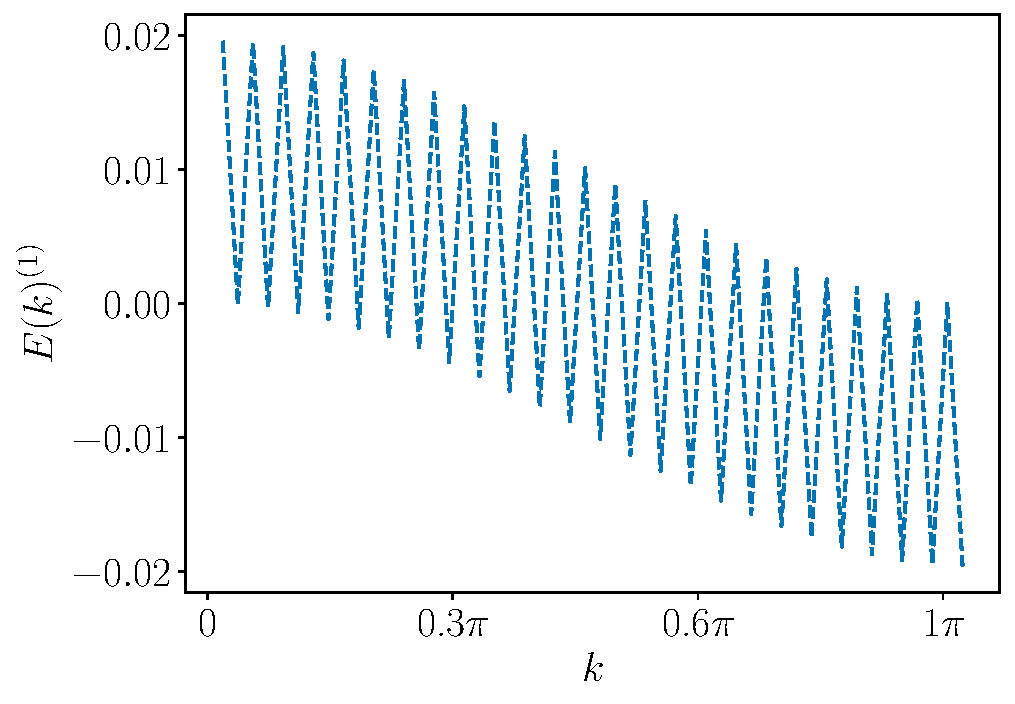
\includegraphics[width=0.5\linewidth]{figures/report_07_2025/E1_corr=50_Omega=0.5_t=0.4.pdf}
        \caption{First order corrections to the energy for a system with 50 sites in the QPC.}
\end{figure*}\label{fig:E1}

To second order one must calculate
\begin{align}
    E_{\nu}^{(2)}(k) & = \sum_{(\mu,p)\neq(\nu,k)} \frac{\left|\bra{\phi^{(0)}_\mu (p)}H_1 \ket{\phi^{(0)}_\nu (k)}\right|^2}{ E_{\nu}^{(0)}(k) -  E_{\mu}^{(0)}(p)}\\
    & = \frac{1}{(N+1)^2}\sum_{(\mu,p)\neq(\nu,k)} \frac{ \xi(k,p)^2}{ E_{\nu}^{(0)}(k) -  E_{\mu}^{(0)}(p)}
\end{align}
where the summation over the $\mu$ and $p$ states is subject to the condition that 
both cannot be equal to $\nu$ and $k$ at the same time. To simplify the calculation,
 it is convenient to separate the sum into three terms
\begin{align}\label{eq:E2}
    E_{\nu}^{(2)}(k) & = \frac{1}{(N+1)^2}\sum_{p\neq k} \left \{ \frac{ \xi(k,p)^2}{ -2J( \cos k - \cos p ) } +  \frac{ \xi(k,p)^2}{ 2\epsilon_\nu -2J( \cos k - \cos p ) } \right \} + \frac{1}{(N+1)^2} \frac{\xi(k,k)^2}{2\epsilon_\nu},
\end{align}
where the first term corresponds to $\mu = \nu, p\neq k$, the second to $\mu \neq \nu, p\neq k$ and the third to $\mu \neq \nu, p = k$. Notice that there are two types of degeneracies in this expression: when $k$ gets close to the boundaries of the band at $0, \pi$ , and when $\epsilon_\nu = -2 J( \cos k -\cos p)$, i.e. the band gap becomes equal to the difference in momentum energies. We shall discuss these in the following after calculating the corrections to the eigenstates. 

The first order corrections to the eigenstates 
\begin{align}
    \ket{\phi_\nu^{(1)} (k)} = \sum_{(\mu,p)\neq(\nu,k)} \frac{\bra{\phi^{(0)}_\mu (p)}H_1 \ket{\phi^{(0)}_\nu (k)}}{ E_{\nu}^{(0)}(k) -  E_{\mu}^{(0)}(p)} \ket{p}\otimes \ket{\mu}.
\end{align} 
are also simpler to calculate by separating it in three contributions
\begin{align}\label{eq:psi_1}
    \ket{\phi_\nu^{(1)} (k)} = & \frac{1}{(N+1)}\sum_{p\neq k} \ket{p}\otimes \left \{ \frac{ \xi(k,p)}{ -2J( \cos k - \cos p ) } \ket{\nu} + \overbrace{\frac{ \xi(k,p)^2}{ 2\epsilon_\nu -2J( \cos k - \cos p )} \ket{\mu}}^{\text{Band mixing term}} \right \} \nonumber \\ 
    & + \frac{1}{(N+1)} \frac{\xi(k,k)}{2\epsilon_\nu} \ket{k}\otimes\ket{\mu},
\end{align}
corresponding to the same ones from Eq.\eqref{eq:E2}. Here, it is important to point out the convention of $\mu \neq \nu$ when it appears explicitly. This convention is held for the rest of this text.

Now, working with Eq.\eqref{eq:psi_1} it is easier to understand what the aforementioned degeneracies mean. The first term, mixes momentum states within the same band and becomes degenerate towards the edges ($k\approx 0, \pi$) due to the cosine shape of the QPC energies. This term will \textit{not} contribute towards the hybridization of the bands. 

On the other hand, the second term is more interesting. It mixes momentum states from different bands ($\nu$ and $\mu$), and becomes degenerate when the difference of between the QPC energies is equal to the band-gap, which can happen at several momenta. If $\nu = +$ the denominator blows up when $p=\pm \arccos(-t/J + \cos k)$ and for $\nu = -$ it happens when $p=\pm \arccos(t/J + \cos k)$. Furthermore, the dependence on the $\arccos$ imposes additional restrictions to the momenta that can cause a degeneracy. Since it is only defined for an argument between $-1$ and $1$, the only states that contribute are those that fulfill:

\begin{tcolorbox}[title=Arccosine condition, colback=white, colframe=black]
Only $k$-momenta that fulfill
\begin{align}\label{eq:arccos_condition}
    -1 + \frac{t}{J} < \cos k < 1 - \frac{t}{J}.
\end{align}
can keep the argument of $p=\pm \arccos(\pm t/J + \cos k)$ between $(-1,1)$. Thus, the corresponding degenerate $p$ will be a physical state.
\end{tcolorbox}

This condition shows that, at larger values of $t$, there will be less available states that can become degenerate and hybridize the two bands. For example, if $t/J\rightarrow 1$, then $|-1+t/J|\rightarrow 0$ and only $k\approx 0,  \pi$ will have a corresponding degenerate $p$, hence only states towards the band edges will mix.

In addition, from the second term it is inferred where is the expansion well-behaved. The trivial answer is when $t>J$, however this regime is not interesting for our purposes. If we are to remain within the small $t$ region, one would have to guarantee $2 |\epsilon_\nu| < \Delta E(k) = -2J(\cos k - \cos(k-\delta))$ at any $k$. This is a very restrictive condition near the boundaries of the gap, but it is much better around $k\approx \pi/2$, when $\Delta E(k)$ is near its maximum. Doing a Taylor expansion of $\Delta E(k)$ around $\pi/2$, where $\delta = \pi/(N+1)$ yields
\begin{align}
    \Delta E(k) \approx k - (k - \delta) = \frac{\pi}{N+1},
\end{align}
so the condition to avoid degeneracies around $\pi/2$ is
\begin{tcolorbox}[title=Non-degeneracy condition, colback=white, colframe=black]
    For momenta near the middle of the band
\begin{align}\label{eq:degen_condition}
    \frac{t}{J}<\frac{\pi}{N+1}, \quad \text{ For $k\approx\pi/2$ }
\end{align}
    guarantees that the perturbative series is well-behaved.
\end{tcolorbox}

On the other hand, if we expand $\Delta E(k)$ around $0$ or $\pi$ we obtain
\begin{align}
    \frac{t}{J}<\left(\frac{\pi}{N+1}\right)^2,
\end{align}
which is specially difficult to achieve for long chains.  Consequently, even if Eq.\eqref{eq:degen_condition} is fulfilled, states far from $k=\pi/2$ will still be degenerate and will present mixing between bands.

\subsection{Comparison to numerical exact diagonalization}

By using both Eq.\eqref{eq:arccos_condition} and \eqref{eq:degen_condition} it is possible to explain the exact diagonalization results in figure \ref{fig:exact_diagonalization}. There, the numerical eigenenergies where sorted into bands according to the overlap matrix between the $H_0$ and $H$ eigenstates
\begin{align}
    O_{i,j} = \bra{\phi_\nu^{(0)}(k)}\ket{\phi_\nu(k)},
\end{align}
where $\ket{\phi_\nu(k)}$ are the full eigenstates of the interacting system. In addition, the color corresponds to the expectation value
\begin{equation}
   \langle P_+\rangle= \bra{\phi_\nu (k)}P_{+}\ket{\phi_\nu (k)} = \bra{\phi_\nu (k)}(\Id_{QPC}\otimes\ket{+})(\Id_{QPC}\otimes\bra{+})\ket{\phi_\nu (k)},
\end{equation}
where $P_+$ is the projection onto the symmetric state of the qubit. In the decoupled case $\langle P_+\rangle$ would be either $0$ or $1$, but once the perturbation is included, it can take any value between $0$ and $1$ depending on whether the state is closer to being antisymmetric or symmetric.

Figure \ref{fig:exact_diagonalization}(a) shows an example where $t>\pi/(N+1)$, where the bands hybridize strongly towards the middle of the band. This is in consistent with Eq.\eqref{eq:degen_condition}, which predicts that the band-mixing term is degenerate even close to $\pi/2$. The fact that the edge states do not mix as much is explained by Eq.\eqref{eq:arccos_condition}: due to the large $t$, would-be-degenerate momenta close to the edges of the band do not fulfill the arccosine condition and are unphysical.

On the other hand \ref{fig:exact_diagonalization}(b) depicts the case when  $t<\pi/(N+1)$ and it shows that states towards the middle of the band remain unmixed, in contrast to the near-edge states. This is expected as the states with $k\approx \pi/2$ fulfill Eq.\eqref{eq:degen_condition}, so band-mixing terms remain small in that region. However, since $\Delta E^{(0)}(k)$ is smaller near the edges, the corresponding states become degenerate and contribute towards band-mixing. Finally, momenta almost at $0$ or $\pi$ remain unmixed due to the arccosine condition Eq.\eqref{eq:arccos_condition}, by the same argument as the previous example.

\begin{figure}[h]
    \centering
    \begin{subfigure}[b]{0.4\textwidth}
        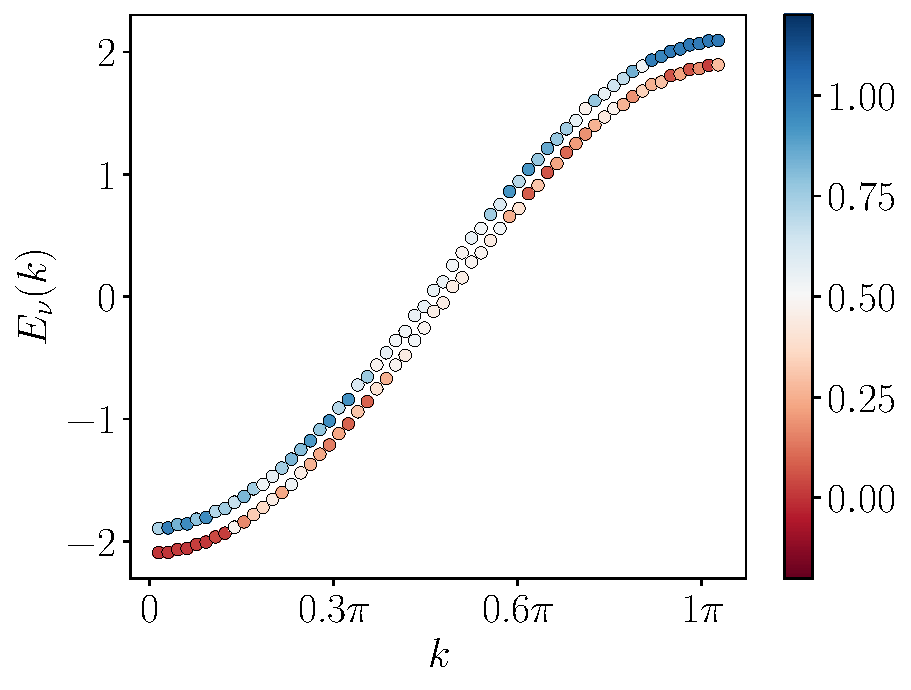
\includegraphics[width=\textwidth]{figures/report_07_2025/exact_energies_Lqpc=60_Omega=0.7_t=0.1.pdf}
        \caption{}
    \end{subfigure}
    \hspace{0.001\textwidth}
    \begin{subfigure}[b]{0.4\textwidth}
        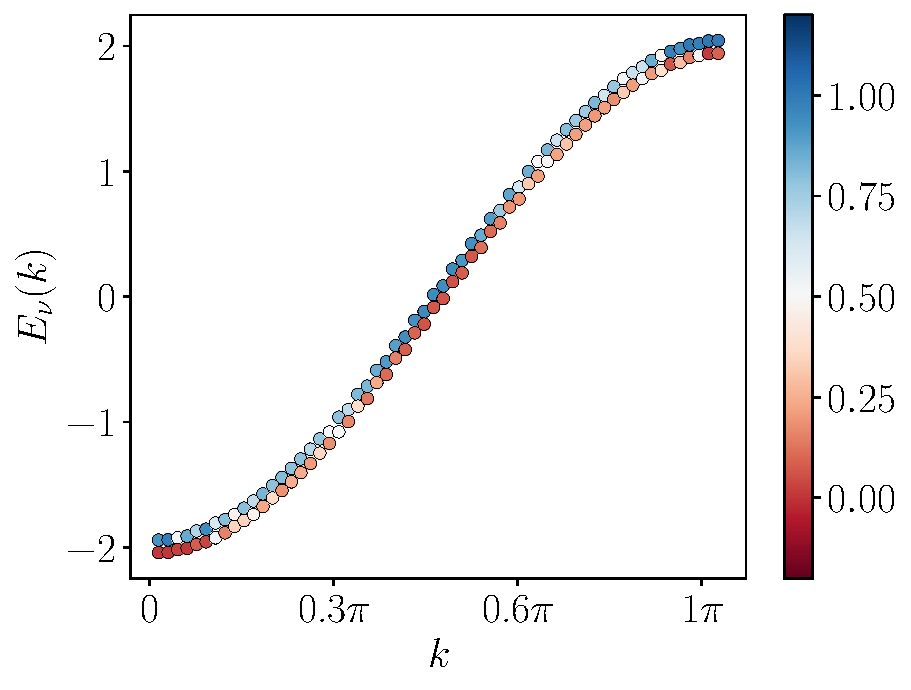
\includegraphics[width=\textwidth]{figures/report_07_2025/exact_energies_Lqpc=60_Omega=0.7_t=0.05.pdf}
        \caption{}
    \end{subfigure}
    \caption{Energy spectrum of the full interacting Hamiltonian $H = H_0+\Omega H_1$ obtained by numerical exact diagonalization. The color corresponds to the projection onto the symmetric non-perturbed eigenstate. Both figures correspond to a system with $N=60$, $\Omega = 0.7$, and $J=1$. Plot (a) has $t=0.1$ and (b) $t=0.05$.}
    \label{fig:exact_diagonalization}
\end{figure}

To summarize: The free Hamiltonian $H_0$ has and antisymmetric and a symmetric band due to the qubit. Turning on the perturbation $H_1$, which couples the momentum of the QPC to the density of the qubit, creates terms that mix momentum states between the two bands, as seen in Eq.\eqref{eq:psi_1}. This expansion becomes degenerate if the band gap $2\epsilon_\nu$ is equal to the energy difference between momenta $\Delta E^{(0)}(k)$, which dictates how the bands hybridize. Towards the middle of the bands ($k\approx \pi/2$) the expansion is well-behaved if Eq.\eqref{eq:degen_condition} is met, thus there is little mixing. On the other hand, close the edges $\Delta E^{(0)}(k)$ is much smaller and these states are degenerate, resulting in strong mixing. Furthermore, there is an additional effect due to Eq.\eqref{eq:arccos_condition} dictatin that states very close to the edge are degenerate with momenta that are not physical, hence they do not mix either. This regime of small $\epsilon$ and $k\approx\pi/2$ is precisely the scattering regime we are most interested in.

\subsection{Corrections to the Reduced Density Matrix}

Perturbative correction to the qubit reduced density matrix are obtained from Eq.\eqref{eq:psi_1}. For a specific eigenstate, the density matrix of the composite system is 
\begin{align}
    \rho(\nu,k) & = \left( \ket{\phi_\nu^{(0)}(k)} + \Omega \ket{\phi_\nu^{(1}(k)} \right)\left( \bra{\phi_\nu^{(0)}(k)} + \Omega \bra{\phi_\nu^{(1}(k)} \right) \nonumber \\
                & = \ket{\phi_\nu^{(0)}(k)}\bra{\phi_\nu^{(0)}(k)} + \Omega \left( \ket{\phi_\nu^{(0)}(k)}\bra{\phi_\nu^{(1)}(k)} + \ket{\phi_\nu^{(1)}(k)}\bra{\phi_\nu^{(0)}(k)}   \right) + \mathcal{O}(\Omega^2),
\end{align} 
from which the qubit density matrix is obtained by $\rho_q(\nu,k) = \sum_m \bra{m}\otimes\Id_q \, \rho(\nu,k)\, \Id_q \otimes\ket{m}$, where $m$ runs over the QPC momenta. 
 
The $\ket{\phi_\nu^{(0)}(k)}\bra{\phi_\nu^{(0)}(k)}$ term yields the pure qubit density matrix. The cross terms are of the form 
\begin{align}
    \sum_{m} \bra{m} \ket{\phi_\nu^{(0)}(k)}\bra{\phi_\nu^{(1)}(k)} \ket{m} = \frac{\xi(k,k)}{2\epsilon_\nu(N+1)}\ket{\nu} \bra{\mu},
\end{align}
where we used the orthogonality $\bra{m}\ket{k}=\delta_{m,k}$ to cancel out the other terns. We stress that $\mu\neq \nu$ always by our convention. 

The qubit density matrix for the $\nu, k$ eigenstate is
\begin{align}
    \rho_{q}(\nu,k) = \ket{\nu}\bra{\nu} + \frac{\Omega \xi (k,k)}{2\epsilon_\nu (N+1)}\left( \ket{\nu} \bra{\mu} + \ket{\mu} \bra{\nu}  \right),
\end{align}
which is appropriate when the system is not in a superposition. We are, however interested in cases where the QPC particle is a Gaussian wavepacket and the qubit is in a general two level state. When there is no perturbation, the corresponding density matrix is of the form
\begin{align}
    \rho^{(0)} = \sum_{k,\nu} | \lambda^{(0)}_{\nu}(k)|^2  \ket{\phi_\nu^{(0)}(k)}\bra{\phi_\nu^{(0)}(k)}
\end{align}
where the probabilities $ \lambda^{(0)}_{\nu}(k) = \alpha (k, k_0) \beta_{\nu}$ are in terms of the Gaussian distribution
\begin{align}
    \alpha(k,k_0) \propto e^{\frac{(k-k_0)^2}{2\Delta^2} + i k x_b}
\end{align}
and qubit probabilities $\beta(\pm)$. It is important to note that, $\alpha(k,k_0)$ is the \textit{discrete} Fourier transform of the Gaussian probability in the lattice basis $\alpha (x,x_b)$ (where $b$ is the bond index) and it will only be a Gaussian itself if we choose $N$ large enough. In general, when the perturbation is turned on, the probabilities will change $| \lambda_{\nu}(k)|^2  \neq | \lambda^{(0)}_{\nu}(k)|^2$. In order to calculate corrections perturbatively, one would have to solve an expansion 
\begin{align}
    \rho(\nu,k) = \rho^{(0)}(\nu,k) + \Omega \rho^{(1)}(\nu,k)
\end{align} 
where \sj{(This part is still a bit fuzzy for me)}
\begin{align}
    \rho^{(1)}(\nu,k) = \sum_{k,\nu} | \lambda^{(0)}_{\nu}(k)|^2  \left(\ket{\phi_\nu^{(0)}(k)}\bra{\phi_\nu^{(1)}(k)} + \ket{\phi_\nu^{(1)}(k)}\bra{\phi_\nu^{(0)}(k)}\right),
\end{align}
such that, the eigenvalues are the probabilities and its corrections are calculated in the same way as usual perturbation theory. To first order 
\begin{align}
    | \lambda^{(1)}_{\nu}(k)|^2 = \bra{\phi_\nu^{0}(k)} \rho^{(1)}(\nu,k)\ket{\phi_\nu^{0}(k)} = 0
\end{align}
due to the $\rho^{(1)}(\nu,k)$ structure. Therefore, it is reasonable to assume that after turning on the perturbation, the superposition probabilities remain largely unchanged and the qubit-QPC system is in the state
\begin{align}
    \ket{\psi} =  \sum_{k,\nu} \lambda^{(0)}_\nu (k)\left( \ket{\phi_\nu^{(0)}(k)} + \Omega \ket{\phi_\nu^{(1}(k)} \right).
\end{align}
The density matrix $\rho = \ket{\psi}\bra{\psi}$ will have cross-terms in $k$ and $\nu$. To simplify this calculation and avoid great pain, we assume that each momentum contributes independently and we take the Gaussian average at the very end, much like is done in scattering problems \cite{shankarQuantumMechanics1994}. In this approximation, the density matrix will be given by
\begin{align}
    \bar{\rho} = \sum_k |\alpha(k,k_0)|^2 \ket{\psi(k)}\bra{\psi(k)}
\end{align}
where $\ket{\psi(k)} = \beta_{+}\ket{\phi_{+}(k)}+\beta_{-}\ket{\phi_{-}(k)}$ and $\ket{\phi_{\nu}(k)} = \ket{\phi^{(0)}_{\nu}(k)}+ \Omega\ket{\phi^{(1)}_{\nu}(k)}$ as we have already calculated. The density matrix will have four terms, where the QPC degrees of freedom are traced out. The resulting qubit density matrix (before the Gaussian averaging) is 
\begin{align}
\rho_q & = \overbrace{|\beta_+|^2 \ket{+}\bra{+} + |\beta_-|^2\ket{-}\bra{-} + \beta_{+}\beta_{-}^* \ket{+}\bra{-} + \beta_{+}^*\beta_{-}\ket{-}\bra{+}}^{\rho_{q}^{(0)}}\nonumber \\
& + \frac{\Omega \xi(k,k)}{2t(N+1)}\underbrace{\left\{ ( |\beta_+|^2 - |\beta_{-}|^2 ) \left( \ket{+}\bra{-} + \ket{-}\bra{+}\right) - \left( \beta_{+}\beta_{-}^* +  \beta_{+}^*\beta_{-} \right)  \left( \ket{+}\bra{+} -  \ket{-}\bra{-}  \right)    \right\}}_{\rho^{(1)}_q}.
\end{align}
A more compact form is found in the $0,1$ basis
 \begin{align}
    & \ket{+} = \frac{1}{\sqrt{2}}\left(\ket{0} +  e^{i\phi}\ket{-}\right), \quad \ket{-} = \frac{1}{\sqrt{2}}\left(\ket{0} +  e^{i\phi}\ket{-}\right)\\
    & \Rightarrow \beta_0 = \frac{1}{\sqrt{2}}( \beta_+ + \beta_{-}), \quad \beta_1 = \frac{e^{i\phi}}{\sqrt{2}}( \beta_+ - \beta_{-}).
 \end{align}
In explicit matrix form
 \begin{align}
    \rho_q^{(0)} = \begin{pmatrix}
        |\beta_0|^2 & \beta_0\beta_1^* \\
        \beta_0^*\beta_1 &  |\beta_1|^2
    \end{pmatrix}, \quad  
    \rho_q^{(1)} = \begin{pmatrix}
        e^{i\phi} \beta_0\beta_1^* + e^{-i\phi} \beta_0^*\beta_1 & - (|\beta_0|^2 - |\beta_1|^2)e^{-i\phi} \\
        - (|\beta_0|^2 - |\beta_1|^2)e^{i\phi} &  - e^{i\phi} \beta_0\beta_1^* - e^{-i\phi} \beta_0^*\beta_1
    \end{pmatrix},
 \end{align}
  it becomes clear that $\rho_q^{(1)}$ is a valid perturbation as $\Tr{\rho_q^{(1)}}=0$ and $(\rho_q^{(1)})^\dagger = \rho_q^{(1)}$. Now, taking the Gaussian average yields
  \begin{align}
    \bar{\rho}_q & = \sum_k |\alpha(k,k_0)|^2 \left(\rho_q^{(0)}   + \frac{\Omega \xi(k,k)}{2t(N+1)}\rho_q^{(1)} \right) \nonumber \\
     & = \rho_q^{(0)}   + \frac{\Omega \bar{\xi}(k_0)}{2t(N+1)}\rho_q^{(1)},
  \end{align} 
where $\bar{\xi}(k_0) =  \sum_k |\alpha(k,k_0)|^2 \xi(k,k)$. 

An even more compact form is obtained by choosing the Bloch representation $\beta_0 = \cos\theta/2$, $\beta_1 = e^{i\phi}\sin\theta/2$ with the Pauli matrices $\sigma_i$
\begin{align}
    \bar{\rho}_q = \frac{1}{2}\left( \Id + \tilde{q}\cdot \vec{\sigma} \right), \quad 
    \tilde{q} = \begin{pmatrix}
        \sin\theta\cos\phi - \frac{\Omega \bar{\xi}(k_0)}{2t(N+1)} \cos\theta \cos\phi\\
        \sin\theta\sin\phi - \frac{\Omega \bar{\xi}(k_0)}{2t(N+1)} \cos\theta \sin\phi \\
        \cos\theta - \frac{\Omega \bar{\xi}(k_0)}{2t(N+1)} \sin\theta 
    \end{pmatrix}.
\end{align}
Unfortunately, the first order corrections to the eigenvalues vanish
\begin{align}
    \tilde{\eta}_{+} = \frac{1}{2}(1\pm|\tilde{q}|) = 1 + \mathcal{O}(\Omega^2), \quad  \tilde{\eta}_{-} = \frac{1}{2}(1\pm|\tilde{q}|) =  \mathcal{O}(\Omega^2),
\end{align}
meaning that, the entanglement entropy also lacks first order corrections and it won't be possible to see mixing between the qubit and the QPC. 

At this point, I am not sure whether this is purely an issue of the order or due to one of the other simplifications. I list them here for convenience:
\begin{itemize}
    \item Truncate to first order in $\Omega$.
    \item The superposition coefficients remain unchanged (true to first order) after turning on the interaction.
    \item Cross momentum terms do not contribute to the reduced density matrix, allowing us to take the Gaussian average at the end. 
\end{itemize}

\bibliography{qpc}
\bibliographystyle{ieeetr}


\end{document}